\section{Date: 2026-09-23}
\noindent \textbf{Series ID: CEU4142000017} 

\noindent This series is titled Indexes of Aggregate Weekly Payrolls of All Employees, Wholesale Trade and has a frequency of Monthly. The units are Index 2007=100 and the seasonal adjustment is Not Seasonally Adjusted.The observation start date is 2006-03-01 and the observation end date is 2026-08-01.The popularity of this series is 1. \\ 

\noindent \textbf{Series ID: ATNHPIUS20100Q} 

\noindent This series is titled All-Transactions House Price Index for Dover, DE (MSA) and has a frequency of Quarterly. The units are Index 1995:Q1=100 and the seasonal adjustment is Not Seasonally Adjusted.The observation start date is 1987-07-01 and the observation end date is 2026-04-01.The popularity of this series is 2. \\ 

\subsection{Raw Regression}
\noindent Regresses the two series against each other directly. A significant result here can come just as easily from both series sharing a long-run trend as from any real relationship.

\begin{center}
\begin{tabular}{lclc}
\toprule
\textbf{Dep. Variable:}             & value\_fred\_ATNHPIUS20100Q & \textbf{  R-squared:         } &     0.731   \\
\textbf{Model:}                     &             OLS             & \textbf{  Adj. R-squared:    } &     0.728   \\
\textbf{Method:}                    &        Least Squares        & \textbf{  F-statistic:       } &     214.8   \\
\textbf{Date:}                      &       Wed, 23 Sep 2026      & \textbf{  Prob (F-statistic):} &  3.06e-24   \\
\textbf{Time:}                      &           15:39:04          & \textbf{  Log-Likelihood:    } &   -377.92   \\
\textbf{No. Observations:}          &                81           & \textbf{  AIC:               } &     759.8   \\
\textbf{Df Residuals:}              &                79           & \textbf{  BIC:               } &     764.6   \\
\textbf{Df Model:}                  &                 1           & \textbf{                     } &             \\
\textbf{Covariance Type:}           &          nonrobust          & \textbf{                     } &             \\
\bottomrule
\end{tabular}
\begin{tabular}{lcccccc}
                                    & \textbf{coef} & \textbf{std err} & \textbf{t} & \textbf{P$> |$t$|$} & \textbf{[0.025} & \textbf{0.975]}  \\
\midrule
\textbf{const}                      &     -11.5081  &       15.435     &    -0.746  &         0.458        &      -42.230    &       19.214     \\
\textbf{value\_fred\_CEU4142000017} &       1.7805  &        0.121     &    14.656  &         0.000        &        1.539    &        2.022     \\
\bottomrule
\end{tabular}
\begin{tabular}{lclc}
\textbf{Omnibus:}       & 32.589 & \textbf{  Durbin-Watson:     } &    0.083  \\
\textbf{Prob(Omnibus):} &  0.000 & \textbf{  Jarque-Bera (JB):  } &    6.325  \\
\textbf{Skew:}          &  0.272 & \textbf{  Prob(JB):          } &   0.0423  \\
\textbf{Kurtosis:}      &  1.744 & \textbf{  Cond. No.          } &     678.  \\
\bottomrule
\end{tabular}
%\caption{OLS Regression Results}
\end{center}

Notes: \newline
 [1] Standard Errors assume that the covariance matrix of the errors is correctly specified.

\begin{figure}
\centering
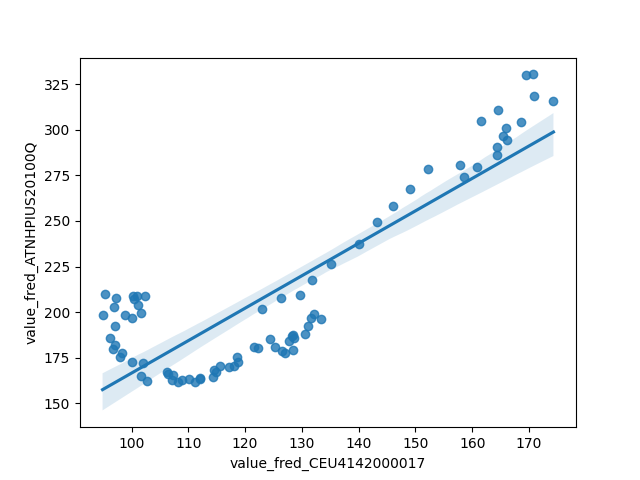
\includegraphics[scale = 0.9]{plots/plot_2026-09-23.png}
\caption{Raw Regression Plot for 2026-09-23}
\end{figure}
\newpage
\subsection{Detrended Regression}
\noindent Regresses the residuals of each series after removing its own linear time trend, so a shared trend can no longer drive the result on its own. A relationship that stays significant here is better evidence of a genuine link between the two series.

\begin{center}
\begin{tabular}{lclc}
\toprule
\textbf{Dep. Variable:}                        & value\_fred\_ATNHPIUS20100Q\_detrended & \textbf{  R-squared:         } &     0.727   \\
\textbf{Model:}                                &                  OLS                   & \textbf{  Adj. R-squared:    } &     0.724   \\
\textbf{Method:}                               &             Least Squares              & \textbf{  F-statistic:       } &     210.7   \\
\textbf{Date:}                                 &            Wed, 23 Sep 2026            & \textbf{  Prob (F-statistic):} &  5.32e-24   \\
\textbf{Time:}                                 &                15:39:04                & \textbf{  Log-Likelihood:    } &   -349.22   \\
\textbf{No. Observations:}                     &                     81                 & \textbf{  AIC:               } &     702.4   \\
\textbf{Df Residuals:}                         &                     79                 & \textbf{  BIC:               } &     707.2   \\
\textbf{Df Model:}                             &                      1                 & \textbf{                     } &             \\
\textbf{Covariance Type:}                      &               nonrobust                & \textbf{                     } &             \\
\bottomrule
\end{tabular}
\begin{tabular}{lcccccc}
                                               & \textbf{coef} & \textbf{std err} & \textbf{t} & \textbf{P$> |$t$|$} & \textbf{[0.025} & \textbf{0.975]}  \\
\midrule
\textbf{const}                                 &   -7.785e-12  &        2.029     & -3.84e-12  &         1.000        &       -4.039    &        4.039     \\
\textbf{value\_fred\_CEU4142000017\_detrended} &       4.4163  &        0.304     &    14.517  &         0.000        &        3.811    &        5.022     \\
\bottomrule
\end{tabular}
\begin{tabular}{lclc}
\textbf{Omnibus:}       &  7.128 & \textbf{  Durbin-Watson:     } &    0.420  \\
\textbf{Prob(Omnibus):} &  0.028 & \textbf{  Jarque-Bera (JB):  } &    3.489  \\
\textbf{Skew:}          &  0.261 & \textbf{  Prob(JB):          } &    0.175  \\
\textbf{Kurtosis:}      &  2.128 & \textbf{  Cond. No.          } &     6.67  \\
\bottomrule
\end{tabular}
%\caption{OLS Regression Results}
\end{center}

Notes: \newline
 [1] Standard Errors assume that the covariance matrix of the errors is correctly specified.

\begin{figure}
\centering
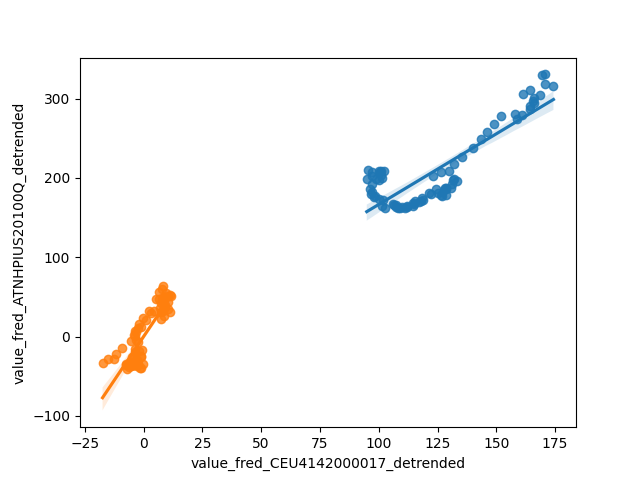
\includegraphics[scale = 0.9]{plots/plot_2026-09-23_detrended.png}
\caption{Detrended Regression Plot for 2026-09-23}
\end{figure}
\newpage
